\apendice{Plan de Proyecto Software}

\section{Introducción}

En este documento se pretende mostrar el plan de proyecto seguido a la hora de realizar el trabajo de fin de grado.

Debido al auge de las metodologías ágiles en la industria y sus indiscutibles ventajas, se ha escogido la metodología \textit{scrum} para desarrollar el proyecto. Los conceptos teóricos seguidos se encuentran en el <<Manual de \textit{scrum}>>~\cite{scrumMaster2022}, temario necesario para obtener la certificación de \textit{Scrum Manager}.

Posteriormente, se expondrá la viabilidad legal y económica del producto.

\section{\textit{Scrum}}

\textit{Scrum} es una metodología ágil basada en cuatro valores~\cite{scrumMaster2022}. Sintetizando sus principios, se puede deducir que se pretende valorar a los individuos por encima de las herramientas, el \textit{software} apropiado a la documentación exhaustiva, la colaboración con el cliente y la habilidad de dar respuesta al cambio ante imprevistos.

Siguiendo este esquema, se desarrolla el <<ciclo de \textit{scrum}>> representado en la imagen~\ref{img:ciclo_scrum}, que se puede dividir en varios pilares.

\begin{figure}[h]
	\caption{Resumen del ciclo de \textit{scrum} según el Manual de \textit{scrum}~\cite{scrumMaster2022}.}
	\label{img:ciclo_scrum}
	\centering
	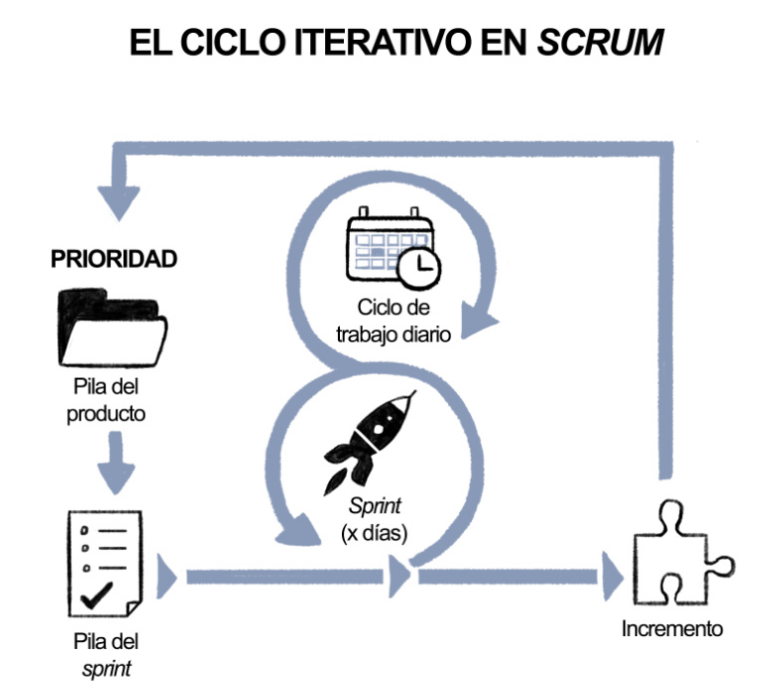
\includegraphics[width=\textwidth]{../img/anexos/scrum/ciclo}
\end{figure}

\subsection{Roles}
Descripción de los posibles interventores durante el desarrollo de un producto.

\begin{itemize}
	\item \textit{Product owner}: es el representante del cliente, y su responsabilidad es el valor del producto. Es quien gestiona la pila del producto (conjunto de historias de usuario solicitadas por el cliente), así como la prioridad de cada ítem que lo compone.
	
	\item \textit{Scrum Master:} es el responsable de garantizar que el proyecto se desarrolla siguiendo los principios de \textit{scrum}, asesorando a los desarrolladores. También es el moderador en las reuniones diarias de \textit{scrum} y el encargado de resolver dinámicas que puedan perjudicar al equipo.
	
	\item \textit{Equipo de desarrollo:} es el conjunto de programadores autogestionados encargados de generar los incrementos. Profesionales multifuncionales, deben completar las tareas que se les asignen en el plazo estimado, además de participar en la toma de decisiones.
\end{itemize}

\subsection{Artefactos}

Son las <<herramientas>>~\cite{scrumMaster2022} elementales. Entre ellos se encuentran:

\begin{itemize}
	\item Pila de producto o \textit{product backlog}: contiene las historias de usuario (el equivalente a los <<requisitos>> en las metodologías tradicionales). Evoluciona durante el proyecto en función de las peticiones del cliente.
	\item Pila del \textit{sprint} o \textit{sprint backlog}: es la lista de tareas que han de completar los desarrolladores en un \textit{sprint}. En este proyecto, se han utilizado las \textit{milestones} de GitHub (asignándoles \textit{issues}) para representarla.
	\item Incremento: resultado de cada \textit{sprint}. Ha de ser un entregable.
	\item Gráfico de avance o \textit{burn down report}: muestra el trabajo pendiente por realizar en un \textit{sprint} y es actualizado por los desarrolladores. Indica, además, el ritmo de trabajo <<ideal>> que se debería seguir para alcanzar los objetivos. En este caso, se ha utilizado el gráfico generado por ZenHub.
	\item Gráfico de producto o \textit{burn up report}: mide cuánto se ha completado respecto al total.
\end{itemize}

\subsection{Eventos}
Durante el ciclo de \textit{scrum}, se pueden identificar varias actividades que constituyen la rutina y se represetan en la imagen~\ref{img:eventos_scrum} facilitada por el Manual de \textit{scrum}~\cite{scrumMaster2022}.

\begin{figure}[h]
	\caption{Eventos de \textit{scrum} según el Manual de \textit{scrum}~\cite{scrumMaster2022}.}
	\label{img:eventos_scrum}
	\centering
	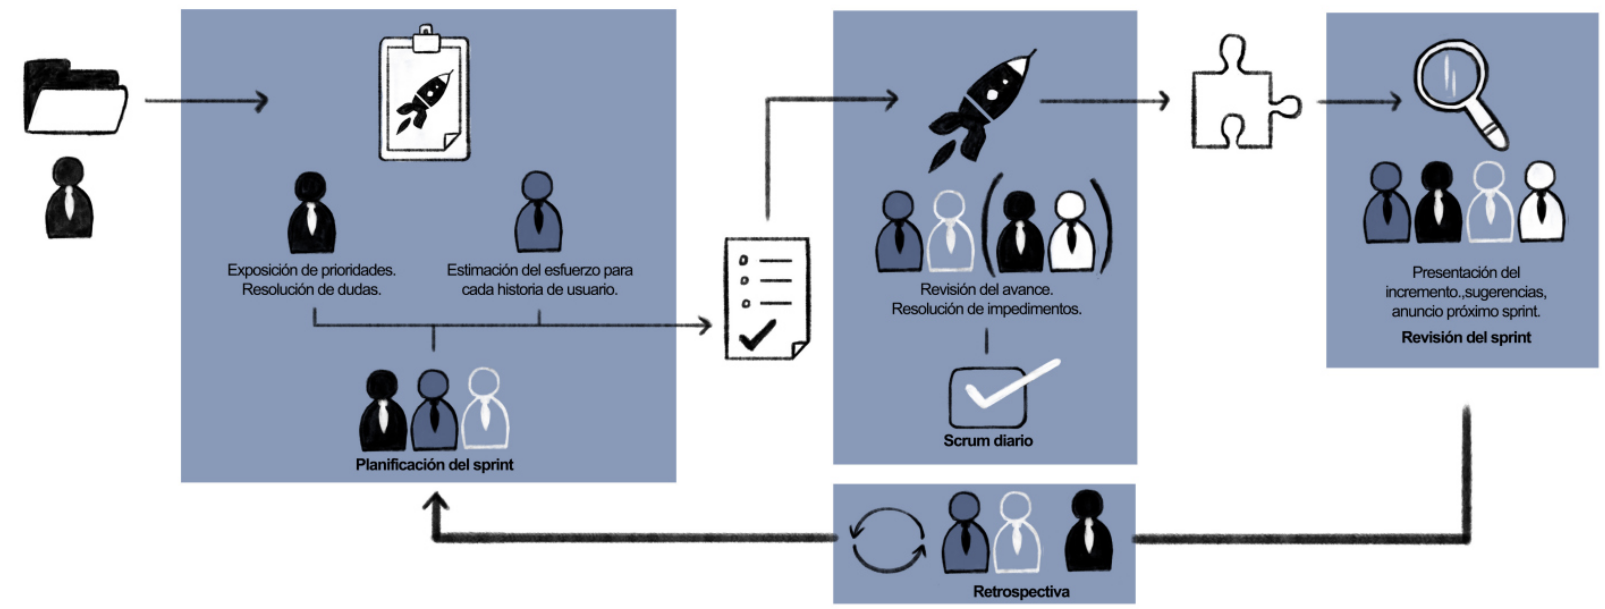
\includegraphics[width=\textwidth]{../img/anexos/scrum/eventos}
\end{figure}

\begin{enumerate}
	\item \textit{Sprint} o iteración: es un periodo de tiempo fijo (y breve) en el que se trabaja para completar una cantidad de tareas prefijadas con antelación (la pila del \textit{sprint}). Se han utilizado los \textit{sprints} de ZenHub para realizar el seguimiento.
	\item Reunión de planificación sel \textit{sprint}: marca el inicio de cada \textit{sprint} y determina las tareas a desarrollar, además de su duración temporal.
	\item\textit{Scrum} diario: breve reunión en la que cada integrante del equipo notifica su ritmo de trabajo con el fin de corregir posibles impedimentos que ralenticen el ciclo. Además, se actualiza el \textit{burndown report}. En este caso, debido a que el equipo está formado únicamente por un desarrollador, se ha omitido.
	\item Revisión del \textit{sprint}: se analiza el incremento entregado y se adapta la pila del producto en caso de necesitarlo (por ejemplo, si se ha encontrado algún \textit{bug} o se necesita refactorizar).
	\item Retrospectiva del \textit{sprint}: se aporta el \textit{feedback} necesario para mejorar la siguiente iteración.
\end{enumerate}

\subsection{Medición}

Como se puede observar, cada equipo puede realizar una cantidad de trabajo, generalmente fija, en cada \textit{sprint}. Por ello, es necesario estimar el tiempo que requiere cada tarea y no asignar más trabajo del que se pueda asimilar en cada iteración.

En este proyecto, se han utilizado los <<puntos de historia>> como unidad de medida.


\section{Planificación temporal}

\subsection{Planificación por \textit{sprints}}

Siguiendo los eventos de \textit{scrum}, y adaptándolos teniendo en cuenta el tamaño del equipo (un desarrollador), se ha decidido planificar el proyecto mediante \textit{sprints}.

\subsubsection{\textit{Sprint 1: Mustard}}

\begin{itemize}
	\item \textbf{\textit{Planning meeting}}
	
	Durante la reunión se marcaron los siguientes objetivos:
	
	\begin{enumerate}
		\item Configuración básica: incluyendo la creación del repositorio, la correcta instalación de ZenHub, la creación de entornos virtuales (miniconda, SKLearn, etc.) y la familiarización con conceptos \textit{scrum}: \textit{milestones, sprints, epics}, etc.
		\item Memoria: comienzo de la redacción incluyendo las secciones de introducción, conceptos teóricos (aprendizaje automático) y trabajo relacionado.
		\item Investigación: búsqueda del código SSADR-CoF y de las bases de datos utilizadas en el paper.
		\item Lectura de papers: Engelen \& Hoos~\cite{engelen2020surveyOnSemiSupervised}, García, Triguero \& Herrera~\cite{triguero2015SelflabeledTechniques}, y Zhou \& Duan~\cite{zhou2021SemisupervisedRecommendationAttack}.
	\end{enumerate}
	
	\item \textbf{Marcas temporales}
	El \textit{sprint} se desarrolló entre el 24 de septiembre de 2022 y el 2 de octubre del 2022.
	
	\item \textbf{\textit{Burndown Report}}
	\begin{figure}[h]
		\caption{\textit{Burndown Report Sprint 01}}
		\centering
		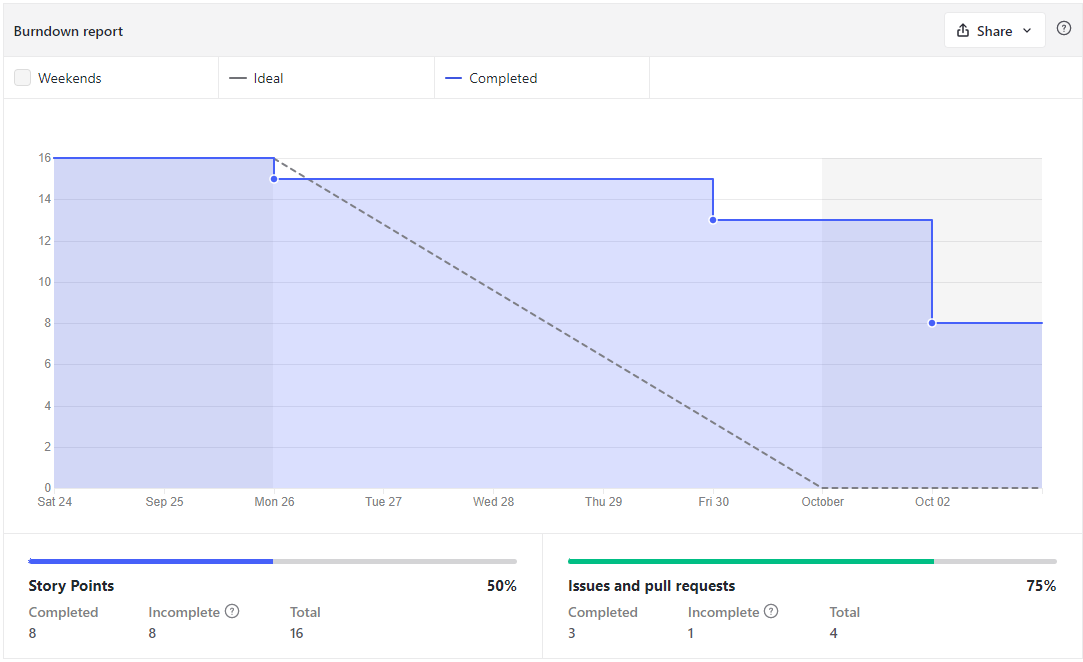
\includegraphics[width=\textwidth]{../img/anexos/bdr/s01_bdr}
	\end{figure}
	
	Como se puede comprobar, no todos los objetivos marcados fueron cumplidos: la estimación del tiempo fue demasiado optimista, además de no contar con el tiempo requerido en solucionar problemas técnicos (\LaTeX{}). Se dejó para próximos sprints la lectura del último paper.

	\item \textbf{\textit{Sprint review meeting}}
	Durante la reunión se fijaron ciertas correcciones en la memoria (mejorar referencias bibliográficas y la sección de <<Trabajos relacionados>>), además de la necesidad de introducir una sección teórica de ataques a los sistemas de recomendación.
	
\end{itemize}


\subsubsection{\textit{Sprint 2: Paprika}}
\begin{itemize}
	\item \textbf{\textit{Planning meeting}}
	Objetivos del siguiente Sprint:
	
	\begin{enumerate}
		\item Configuración: debido a la gran cantidad de tiempo invertida en solucionar errores de compilación en \LaTeX{}, se decidió migrar el proyecto a una nueva instalación basada en Debian.
		\item Correcciones: aspectos estilísticos y completar información.
		\item Lectura: Mingdan y Qingshan~\cite{mingdan2018ShillingAttacksAReview} con el objetivo de introducir una sección teórica de ataques.
		\item Memoria: redacción completa de los modelos de ataque en los aspectos teóricos.
		
	\end{enumerate}
	
	\item \textbf{Marcas temporales}
	El \textit{sprint} se desarrolló entre el 3 de octubre de 2022 y el 18 de octubre del 2022.
	
	\item \textbf{\textit{Burndown Report}}
	\begin{figure}[h]
		\caption{\textit{Burndown Report Sprint 02}}
		\centering
		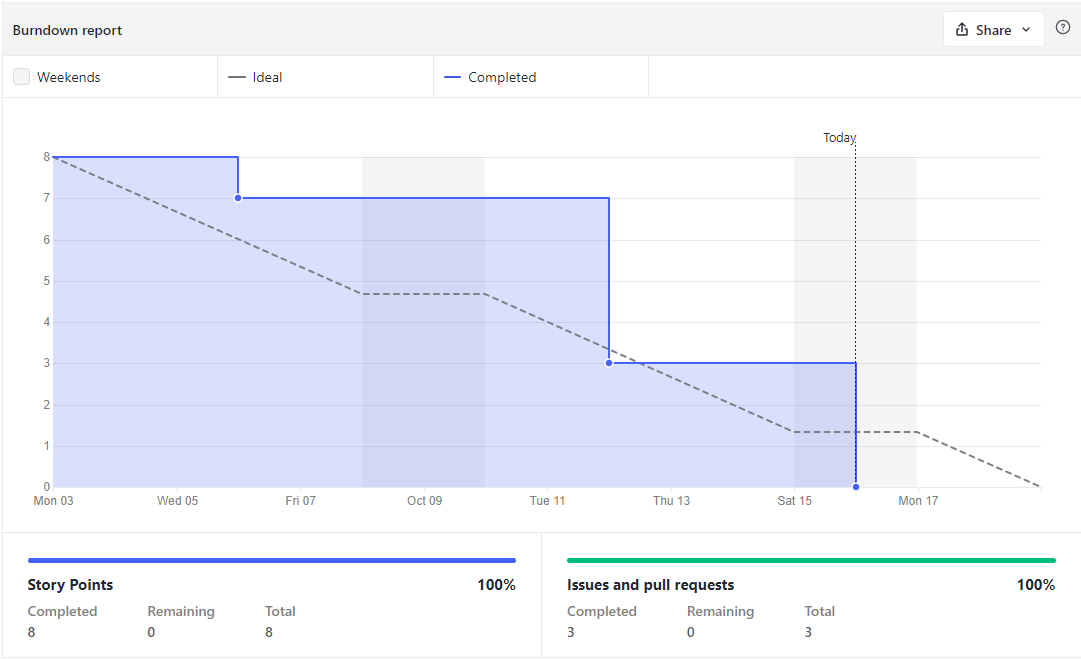
\includegraphics[width=\textwidth]{../img/anexos/bdr/s02_bdr}
	\end{figure}
		
	En este \textit{sprint} sí se cumplió con los objetivos marcados. Sin embargo, la estimación de tiempo tampoco fue la adecuada, requiriendo más de lo previsto.
	\item \textbf{\textit{Sprint review meeting}}
	Durante la reunión se resolvieron dudas acerca de bibliografía, referencias y trabajo previo. Además, se acordó empezar a programar, definiendo así los \textit{issues} desarrollados en el siguiente \textit{sprint}.
	
\end{itemize}

\subsubsection{\textit{Sprint 3: Fennel Seeds}}
\begin{itemize}
	\item \textbf{\textit{Planning meeting}}
	
	Durante esta reunión, se decidió empezar a programar el \textit{co-forest}. Para ello, se definieron los siguientes pasos:
	
	\begin{enumerate}
		
		\item Librerías: se acordó aprender a utilizar las librerías más comunes en el \textit{data science}. Entre ellas: MatplotLib y SKLearn. Además, se requirió la correcta configuración del entorno virtual, haciendo que el tiempo dedicado al \textit{issue} fuese mayor de lo estimado (problemas en el \texttt{PATH} y con las dependencias).
		
		\item \textit{SKLearn}: aprovechando la correcta documentación de la librería, se decidió repasar los conceptos teóricos básicos, además del manejo de la <<interfaz>> (métodos comunes). Entre ellos:
		
		\begin{itemize}
			\item \textit{Decision trees}
			\item \textit{Self training}
			\item \textit{Random Forest}
		\end{itemize}
	
		\item Lectura: se concertó la relectura del artículo de Zhou~\cite{zhou2021SemisupervisedRecommendationAttack} con la intención de comprender el algoritmo y del \textit{paper} <<original>> del \textit{co-forest}~\cite{originalCoForest2007}. Durante el proceso de programación, además, se encontró la tesis de Van Engelen~\cite{engelen2018thesis} y se añadió al conjunto.
		\item Documentación: se acordó la corrección de los errores previamente señalados y la inclusión del \textit{sprint} en los anexos.
		\item Programación del \textit{Co-Forest}: se programó el pseudocódigo ilustrado en la Tesis de Van Engelen~\cite{engelen2018thesis}, que es muy similar al original~\cite{originalCoForest2007} pero con algunas diferencias. Inicialmente se intentó usar el \textit{Random Forest} de \textit{SKLearn}, pero se descartó la idea debido a la poca versatilidad que se ofrecía para manejar los \textit{concomitant ensembles}. Se han de corregir ciertos factores, pero se pospondrá hasta la correcta discusión con el tutor.
		
	\end{enumerate}
	
	\item \textbf{Marcas temporales}	
	El \textit{sprint} se desarrolló entre el 19 de octubre de 2022 y el 2 de noviembre del 2022.
	
	\item \textbf{\textit{Burndown Report}}
	
		\begin{figure}[h]
		\caption{\textit{Burndown Report Sprint 03}}
		\centering
		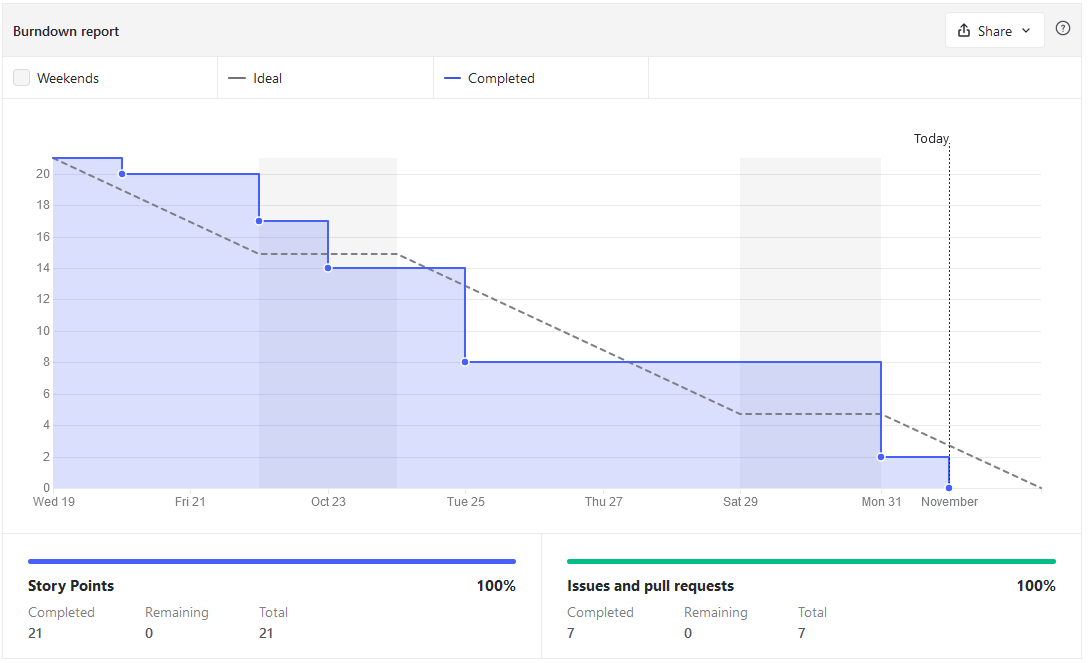
\includegraphics[width=\textwidth]{../img/anexos/bdr/s03_bdr}
		\end{figure}
	
	En este \textit{sprint} se cumplió con los objetivos marcados. Nuevamente, la estimación del tiempo fue inferior a la real (se pensaba que se podría depender más de librerías existentes de lo que se pudo en realidad), calculándose un total de aproximadamente 25 horas reales.

	\item \textbf{\textit{Sprint review meeting}}
	
	Durante la revisión del \textit{sprint}, se llegó a la conclusión de que el pseudocódigo podía ser mejor implementado aprovechando ciertas librerías de \textit{Python}. Se comentó cómo mejorar complejidades espaciales y reducir el código. Se fijaron objetivos para las próximas semanas.
	
\end{itemize}


\subsubsection{\textit{Sprint 4: Cayenne}}
\begin{itemize}
	\item \textbf{\textit{Planning meeting}}
	
	Durante la reunión se acordaron los siguientes objetivos:
	
	\begin{enumerate}
		\item Reimplementación del código: se acordó volver a programar el \textit{co-forest}, esta vez implementando una versión más <<\textit{pythoniana}>> con el fin de mejorar la complejidad espacial y facilitar la lectura.
		\item Curso de Numpy: se decidió que sería interesante la realización de un curso para aprender a utilizar la librería y aplicarla al código.
		\item Curso de Pandas: aprovechando la relación con el punto anterior, se acordó completar también un curso de esta librería.
		\item Memoria: corregir aspectos anteriores e incluir toda la teoría relacionada con el \textit{co-forest}.
	\end{enumerate}
	
	\item \textbf{Marcas temporales}
	El \textit{sprint} se desarrolló entre el 3 de noviembre de 2022 y el 15 de noviembre del 2022.
			
	\item \textbf{\textit{Burndown Report}}
	\begin{figure}[h]
		\caption{\textit{Burndown Report Sprint 04}}
		\centering
		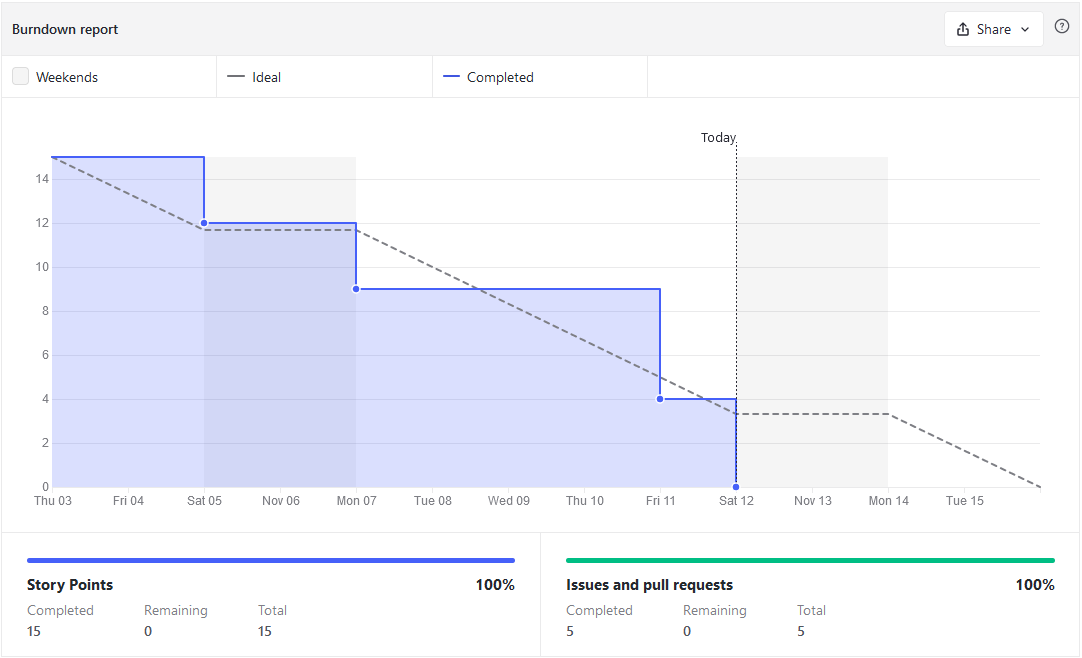
\includegraphics[width=\textwidth]{../img/anexos/bdr/s04_bdr}
	\end{figure}
	
	En este \textit{sprint} se completaron los objetivos, aunque quedaron pendientes ciertos aspectos a comentar respecto al código. Destacar que, debido a que se terminaron antes de lo planeado los \textit{issues} planificados, se aprovechó para modificar ciertos aspectos pendientes relacionados con la memoria y para probar correctamente el código. Esto hizo que el tiempo real dedicado haya sido ligeramente superior al estimado (más tiempo de documentación).
	
	\item \textbf{\textit{Sprint review meeting}}
	En la reunión se acordó experimentar con el algoritmo utilizando distintos conjuntos de datos, además de mejorar ciertos detalles de implementación.
	
\end{itemize}

\subsubsection{\textit{Sprint 5: Curry}}

\begin{itemize}
	\item \textbf{\textit{Planning meeting}}
		Durante la reunión se acordaron los siguientes objetivos:
	
	\begin{enumerate}
		\item Ajustes al código: se acordó mejorar algunos factores, como la generación de objetos <<aleatorios>> para obtener resultados deterministas en los experimentos, optimización de memoria o corrección de parámetros.
		\item Experimentación: se determinó probar el código con distintos conjuntos de datos en diferentes fases: durante el entrenamiento y tras terminarlo. Para ello, se estudiaron algunos conceptos teóricos y el uso de la librería MatplotLib para representar gráficamente los resultados obtenidos.
		\item Memoria: documentación de los experimentos realizados y correcciones.
	\end{enumerate}

	\item \textbf{Marcas temporales}		
	El \textit{sprint} se desarrolló entre el 15 de noviembre de 2022 y el 25 de noviembre del 2022.
	
	\item \textbf{\textit{Burndown Report}}
		\begin{figure}[h]
		\caption{\textit{Burndown Report Sprint 05}}
		\centering
		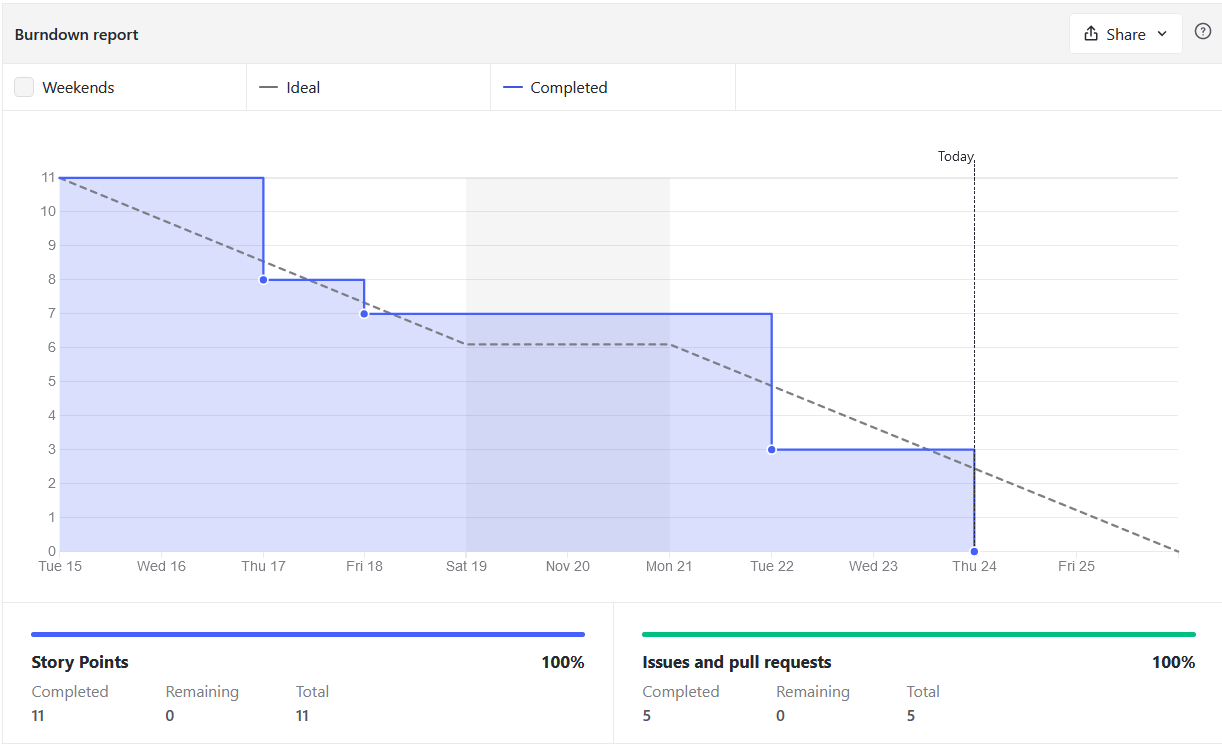
\includegraphics[width=\textwidth]{../img/anexos/bdr/s05_bdr}
	\end{figure}
	
	En este \textit{sprint} se cerraron todos los puntos de historia propuestos. Aunque se estimaron 11 horas de trabajo, el tiempo invertido fue superior, realizando 15. La mayor dedicación se justifica por la existencia de reuniones intermedias y de <<defectos>> encontrados en el código en el trascurso del \textit{sprint}.
	
	\item \textbf{\textit{Sprint review meeting}}
	Durante la reunión se acordó comparar los resultados obtenidos con los de otras herramientas, además de empezar el tratamiento de los conjuntos de datos utilizados en el \textit{paper}~\cite{zhou2021SemisupervisedRecommendationAttack}.
	
\end{itemize}


\subsubsection{\textit{Sprint 6: Coriander}}
\begin{itemize}
	\item \textbf{\textit{Planning meeting}}
	Durante la reunión se fijaron los siguientes objetivos:
	
		\begin{enumerate}
		\item Ajustes en las gráficas: arreglar detalles menores en el formato de ciertos gráficos.
		\item Comparativas: probar los resultados obtenidos y compararlos la herramienta de la Universidad de Granada llamada \textit{Keel}.
		\item \textit{Datasets} <<reales>>: probar el algoritmo utilizando MovieLens, una de las bases de datos utilizadas en el \textit{paper}~\cite{zhou2021SemisupervisedRecommendationAttack}. Para ello, es necesaria una re-lectura del artículo y realizar el procesamiento inicial de los datos.
		\item Memoria: documentación de los experimentos realizados.
	\end{enumerate}

	\item \textbf{Marcas temporales}		
	El \textit{sprint} se desarrolló entre el 25 de noviembre de 2022 y el 5 de diciembre del 2022.
	
	\item \textbf{\textit{Burndown Report}}
		\begin{figure}[h]
			\caption{\textit{Burndown Report Sprint 06}}
			\centering
			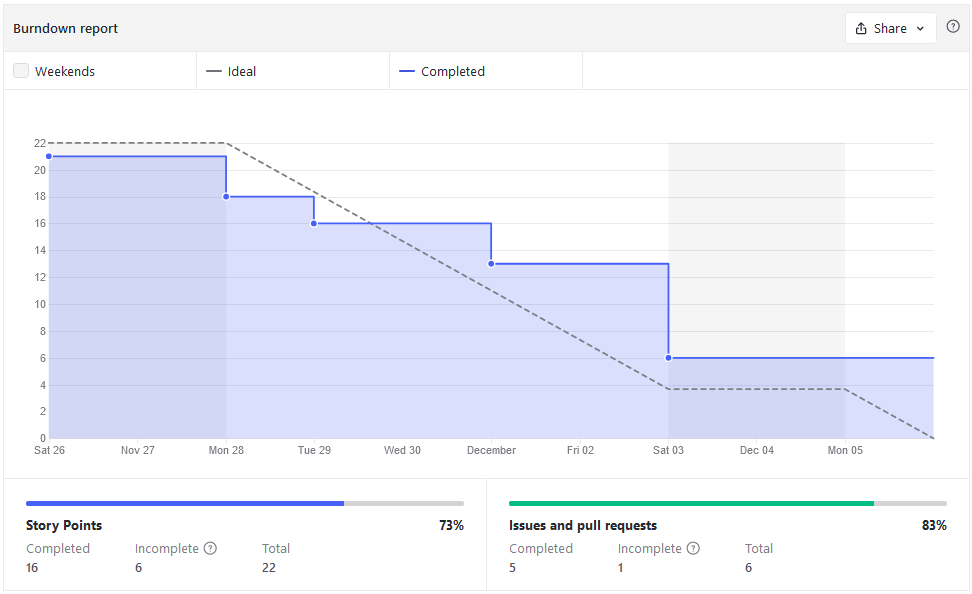
\includegraphics[width=\textwidth]{../img/anexos/bdr/s06_bdr}
		\end{figure}
	
	Puede parecer que los puntos de historia fueron mal estimados debido a que el ritmo de trabajo es bajo. Sin embargo, se justifica debido a que durante la experimentación (en concreto, durante la comparativa contra KEEL) se encontraron dos \textit{bugs} en el código (causados no por la lógica del programa, sino por el operador \textit{in} de Python y por no estar preparado para recibir etiquetas que no comiencen en 0).
	
	Debido a que los errores se encontraron una vez se realizó toda la documentación, se tuvo que repetir la sección asociada a los experimentos del \textit{co-forest}, además de localizar y depurar los errores de código. Todo este trabajo supuso un esfuerzo extra de 7 horas, que fueron introducidas en el \textit{backlog} del \textit{sprint} a mediados del mismo (debido a la gran importancia que tienen y la influencia en pasos posteriores). Por este motivo, no se completaron los objetivos previstos. Sin embargo, el tiempo dedicado al proyecto fue el estimado.
	
	Es destacable también que de los 6 puntos de historia que quedan se realizaron 2, pero se decidió dejar el \textit{issue} abierto para el siguiente \textit{sprint}.

	\item \textbf{\textit{Sprint review meeting}}
	
	Habiendo finalizado el modelo, se decidió empezar a experimentar con bases de datos de sistemas de recomendación. Además, se acordó añadir nuevas gráficas.
\end{itemize}

\subsubsection{\textit{Sprint 7: Cinnamon }}
\begin{itemize}
	\item \textbf{\textit{Planning meeting}}
	
	Se marcaron los siguientes objetivos para el \textit{sprint}.
	
	\begin{enumerate}
		\item Extraer vectores de características: estudiar e implementar el método de extracción de vectores por ventanas expuesto en el \textit{paper} de Zhou y Duan~\cite{zhou2021SemisupervisedRecommendationAttack}. Generar ficheros \texttt{.csv} con dichos vectores para poder importarlos posteriormente con Pandas. Probar la correcta generación de vectores con perfiles verdaderos y atacantes.
		\item Generación de reseñas de atacantes: siguiendo los modelos estadísticos, generar reseñas de ataque para el \textit{random attack}, el \textit{average attack} y el \textit{bandwagon attack}.
		\item Documentación: añadir introducción y descripción de \textit{scrum} en los anexos. Corregir las sugerencias anteriores. Incluir la descripción del método de extracción de vectores de características por ventanas y la generación de reseñas de atacantes.
	\end{enumerate}
	
	\item \textbf{Marcas temporales}		
	El \textit{sprint} se planificó para desarrollarse entre el 8 y el 20 de diciembre de 2022. Sin embargo y debido al ritmo de trabajo, se cerró el 15 de diciembre de 2022.
	
	\item \textbf{\textit{Burndown Report}}
	\begin{figure}[h]
		\caption{\textit{Burndown Report Sprint 07}}
		\centering
		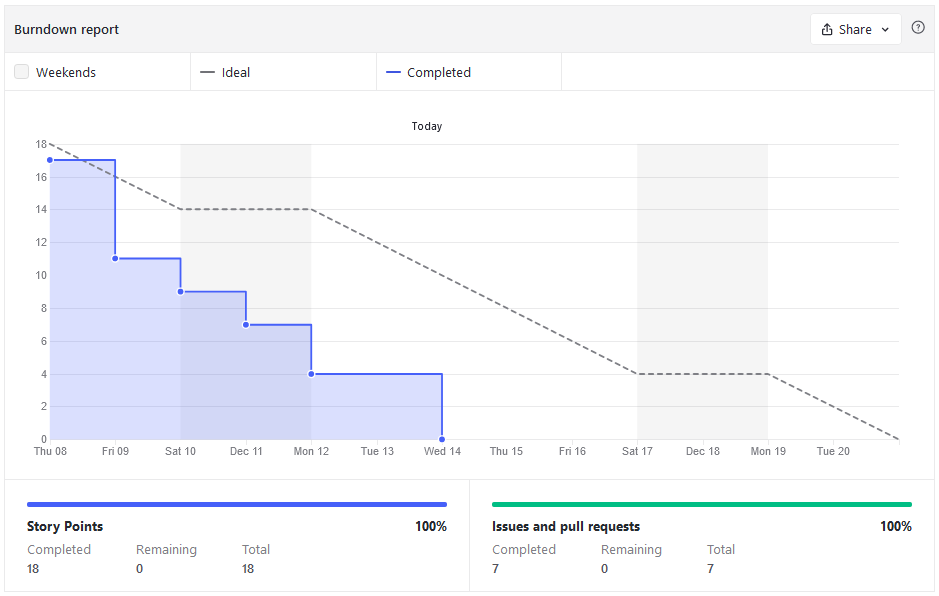
\includegraphics[width=\textwidth]{../img/anexos/bdr/s07_bdr}
	\end{figure}

	Como se puede comprobar, se finalizaron las tareas del \textit{sprint} antes de lo previsto. En gran parte, debido a que el \textit{issue} de extracción de vectores de características estaba ya comenzado en el \textit{sprint} anterior, y requirió menos tiempo del planificado. Además, el resto de tareas no dieron problemas en esta iteración. Debido a que \textit{scrum} no permite añadir nuevos ítems en la pila del \textit{sprint} durante el desarrollo de este, se decidió cerrar y comenzar uno nuevo.

	\item \textbf{\textit{Sprint review meeting}}
\end{itemize}





\subsubsection{\textit{Sprint N: }}
\begin{itemize}
	\item \textbf{\textit{Planning meeting}}
			\begin{enumerate}
			\item
			\item
			\item
			\item 
			\end{enumerate}
	\item \textbf{Marcas temporales}		
	\item \textbf{\textit{Burndown Report}}
	\item \textbf{\textit{Sprint review meeting}}
\end{itemize}
\section{Estudio de viabilidad}

\subsection{Viabilidad económica}

\subsection{Viabilidad legal}


